\documentclass[12pt]{article}
\usepackage{geometry}                % See geometry.pdf to learn the layout options. There are lots.
\geometry{letterpaper}                   % ... or a4paper or a5paper or ... 
%\geometry{landscape}                % Activate for for rotated page geometry
\usepackage[parfill]{parskip}    % Activate to begin paragraphs with an empty line rather than an indent
\usepackage{daves,fancyhdr,natbib,graphicx,dcolumn,amsmath,lastpage,url}
\usepackage{amsmath,amssymb,epstopdf,longtable}
\usepackage[final]{pdfpages}
\DeclareGraphicsRule{.tif}{png}{.png}{`convert #1 `dirname #1`/`basename #1 .tif`.png}
\pagestyle{fancy}
\lhead{CE 5364 -- Groundwater Transport Phenomena }
\rhead{FALL 2025}
\lfoot{ES4}
\cfoot{}
\rfoot{Page \thepage\ of \pageref{LastPage}}
\renewcommand\headrulewidth{0pt}



\begin{document}
\begin{center}
{\textbf{{ CE 5364 Groundwater Transport Phenomena } \\ {Exercise Set 4}}}
\end{center}

\section*{\small{Exercises}}
\begin{enumerate}% Problem Counter
\item Figure \ref{fig:plumemap} below shows a piezometric map for a shallow sand aquifer.\footnote{Problem 2-8, pg. 578 in Bedient, et. al.}  The hydraulic conductivtiy is estimated to be $1.5 \times 10^{-2}~\frac{cm}{s}$, the saturated thickness is 40 feet, and the effective porosity is 0.3.

\begin{figure}[h!] %  figure placement: here, top, bottom, or page
   \centering
   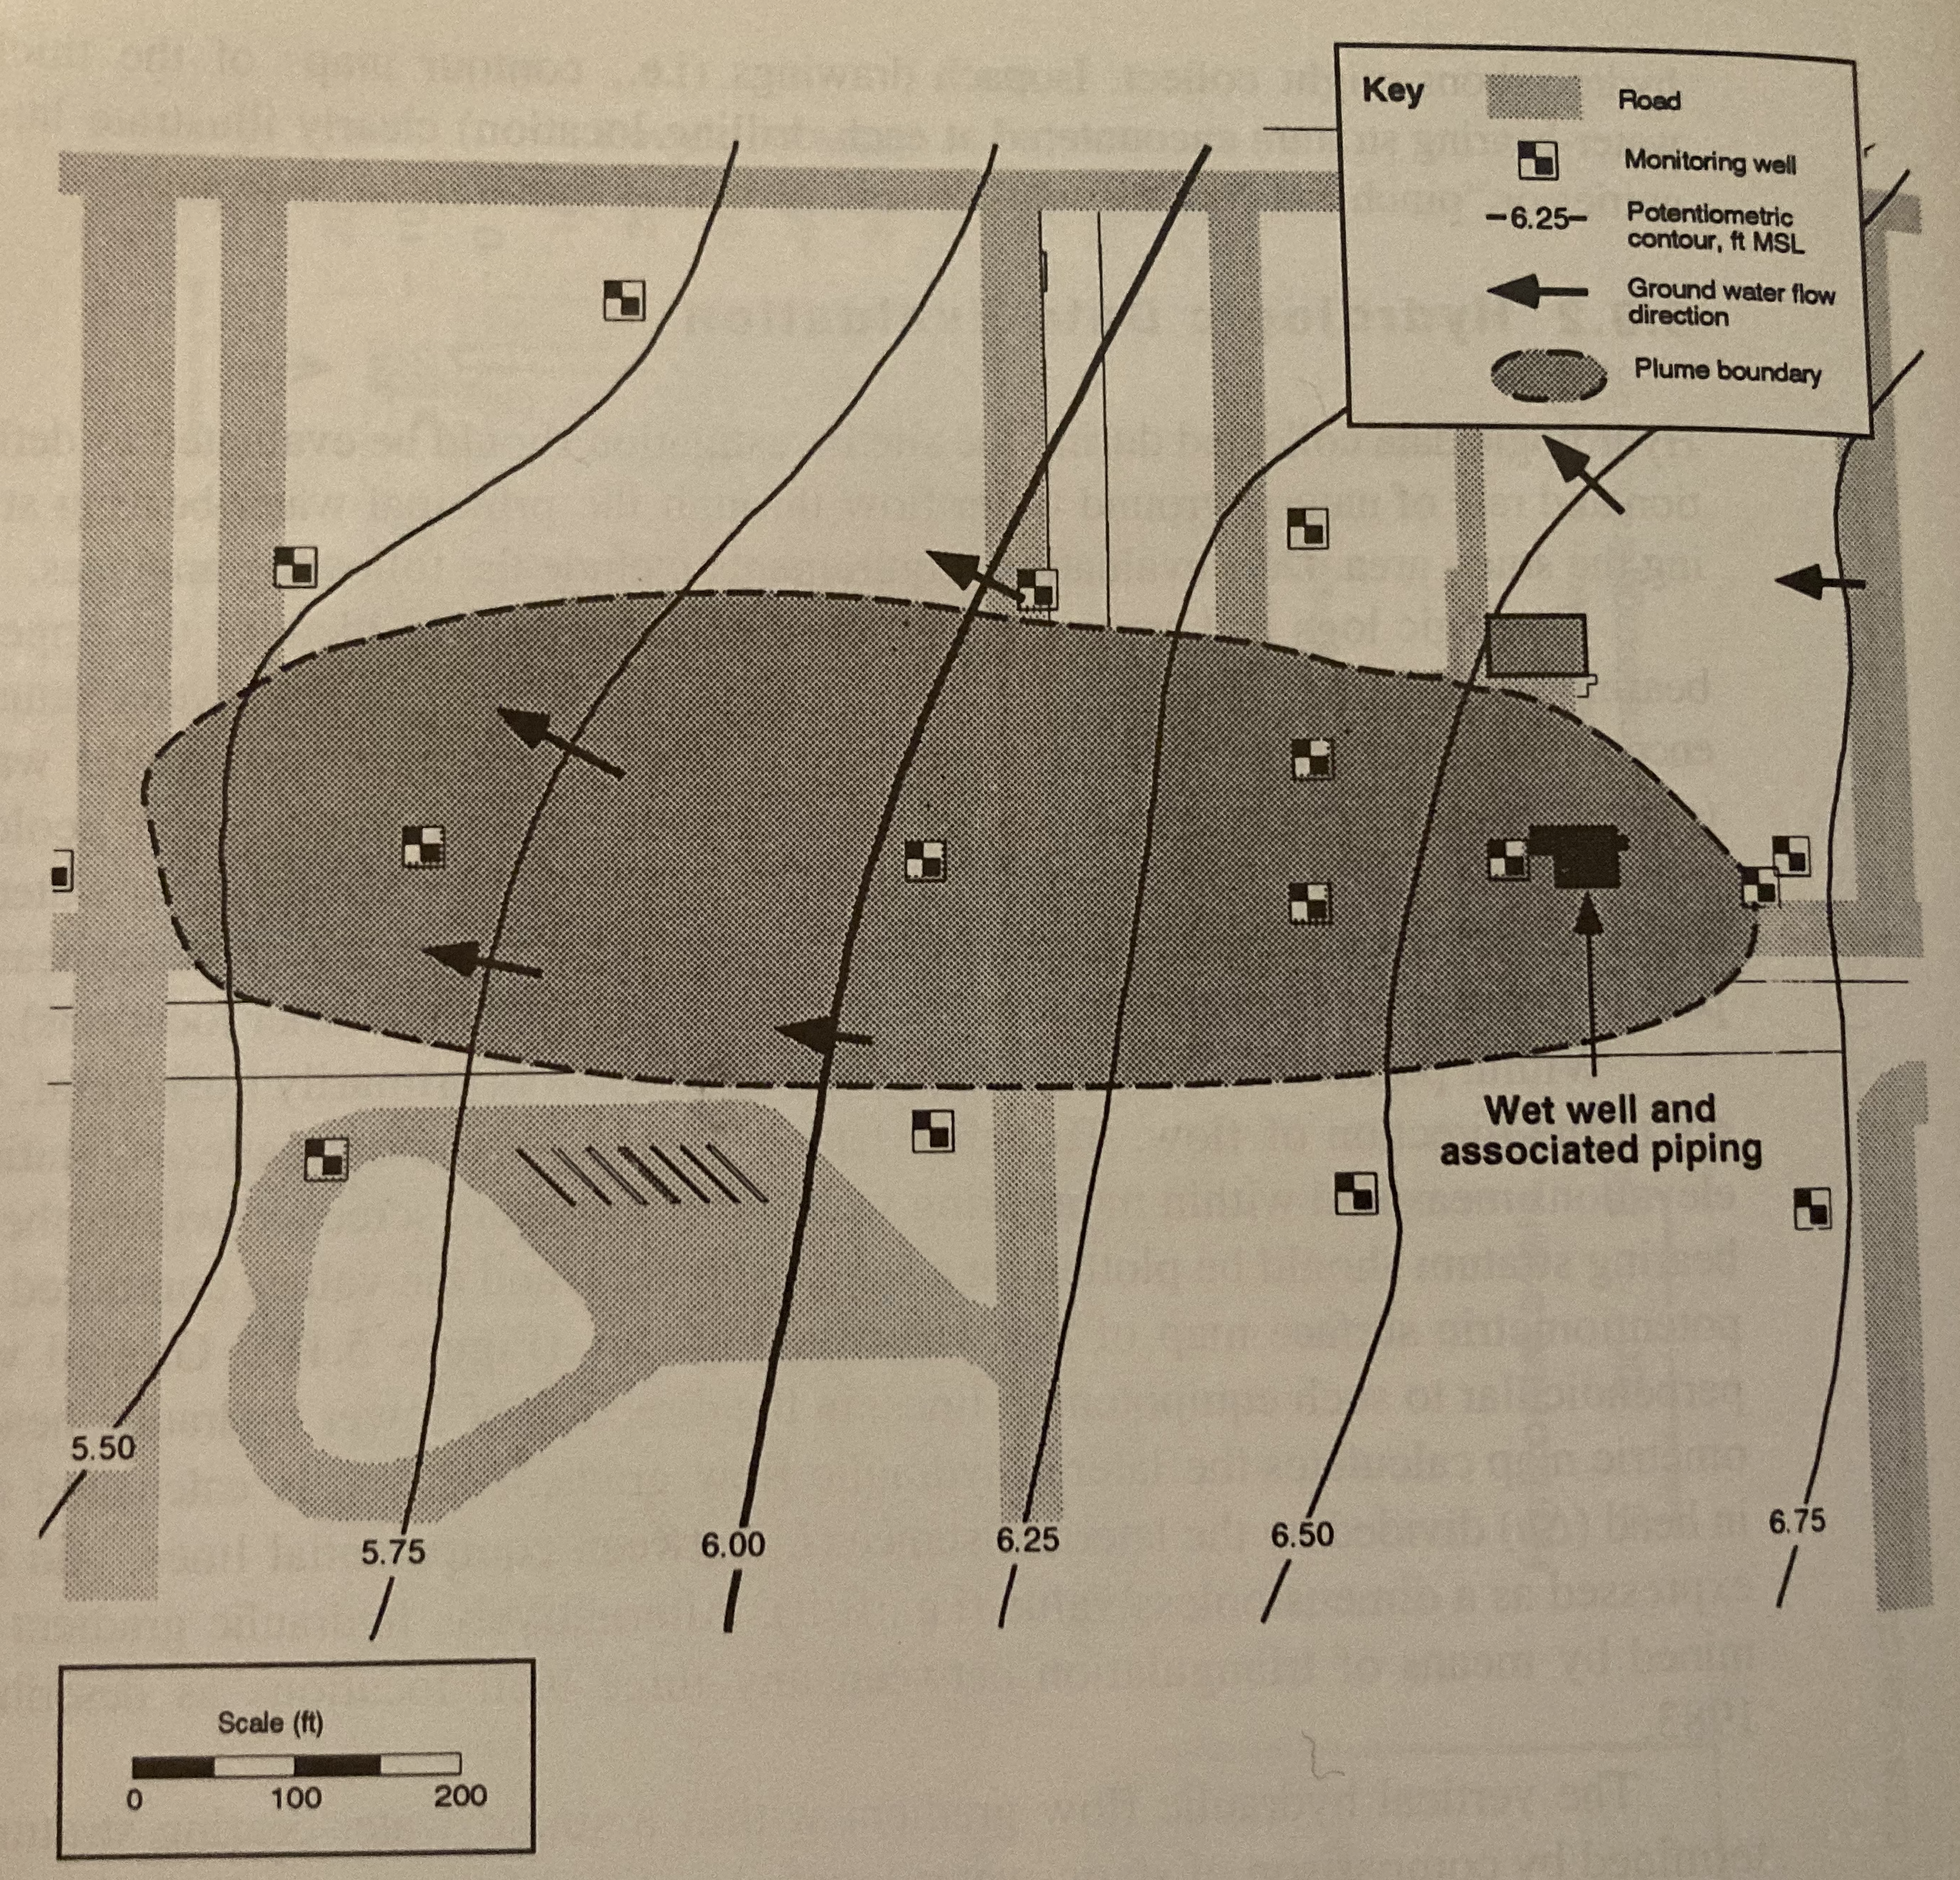
\includegraphics[width=5.5in]{Fig5.18.png} 
   \caption{Plume Map (plan view)}
   \label{fig:plumemap}
\end{figure}

\clearpage
Determine:
\begin{enumerate}
\item A well naming scheme (suggest left to right, bottom to top but any scheme will do so you can identify specific wells)
\item Which well is expected to be the most contaminated.
\item The groundwater velocity and seepage velocity across the plume.
\item The duration (estimate) that the source has been contaminating the aquifer (neglect dispersion, diffusion, and adsorption).
\item The flow rate across the plume.
\item An explaination for contamination upgradient of the source zone.
\end{enumerate}

\end{enumerate}% Problem Counter
\end{document}  